\documentclass[12pt]{article}

\usepackage[german]{babel}
\usepackage{amsmath}
\usepackage{amssymb} % to display symbols for real numbers, integers etc. Usage: \mathbb{R}
\usepackage{graphicx}
\usepackage{listings} % to display programming code
%\usepackage[ngerman]{babel}
\usepackage{color}
\usepackage{relsize} % to display scaled math symbols (big summation symbol etc.)
\usepackage{textcomp}

\DeclareGraphicsExtensions{.pdf,.jpeg,.png}
\definecolor{listinggray}{gray}{0.9}
\definecolor{lbcolor}{rgb}{0.9,0.9,0.9}
\lstset{ % to display programming code in nice colors
	backgroundcolor=\color{lbcolor},
	tabsize=4,
	rulecolor=,
	language=matlab,
		basicstyle=\scriptsize, %for extra small font size
        upquote=true,
        aboveskip={1.5\baselineskip},
        columns=fixed,
        showstringspaces=false,
        extendedchars=true,
        breaklines=true,
        prebreak = \raisebox{0ex}[0ex][0ex]{\ensuremath{\hookleftarrow}},
		frame=single, %draw frame
        showtabs=false,
        showspaces=false,
        showstringspaces=false,
        identifierstyle=\ttfamily,
        keywordstyle=\color[rgb]{0,0,1},
        commentstyle=\color[rgb]{0.133,0.545,0.133},
        stringstyle=\color[rgb]{0.627,0.126,0.941},
        numbers=left,
        stepnumber=1,
        firstnumber=1,
        numberfirstline=true,
        linewidth=14cm,
}

\title{\"Ubungsblatt 6\\ \glqq Mustererkennung\grqq}
\author{J. Cavojska, N. Lehmann, R. Toudic}
\date{16.06.2015}
\begin{document}
\maketitle
%\renewcommand{\contentsname}{Table of Contents}
\tableofcontents
\newpage

\section{Perzeptron Lernalgorithmus}

\begin{lstlisting}[language=Matlab]
% Clean up
clear all
close all
clc

% Datenaufbereitung
Data     = load('klausur.txt');
Punkte   = Data(:,1);
Features = horzcat(Punkte, ones(size(Punkte,1), 1));
Noten    = Data(:,2);
Punkte0  = Data((Data(:,2)==0),:);
Punkte1  = Data((Data(:,2)==1),:);
x1       = linspace(0,1);
x2       = linspace(-5,5);


w = [0 0]; % random choosen vector w
limit = size(Data, 1);  % number of iterations | Abbruchkriterium
for i = 1:limit
    if w(1) == 0 && w(2) == 0
        w_norm = [0 0];
    else
        w_norm = w / norm(w);
    end
    lineNum = mod(i, size(Features,1))+1;
    proj = Features(lineNum, :) * w_norm'; % scalar projection
    
    if Noten(lineNum) == 1
        if proj < 0 % wrong classification
            
            Features(lineNum, :);
            w = w + Features(lineNum, :);
            w_norm = w / norm(w);
            w_x = w(1) * x1;
            
            if w(2) == 0
                w_y = w_x * 0;
            else
                coeff_w = w(2) / w(1)
                w_y = w_x * coeff_w;
            end
            
            diskriminante = [-w(2) w(1)];
            diskriminante_x = diskriminante(1) * x1;
            
            if diskriminante(1) == 0
                diskriminante_y = linspace(0, diskriminante(2));
            else
                coeff_d = diskriminante(2) / diskriminante(1);
                diskriminante_y = diskriminante_x * coeff_d;
            end
            
            % plot
            figure('NumberTitle','off','Name','Aufgabe 1 - Perceptron Learning');
            hold on            
            
            plot(w_x, w_y, 'g');
            plot(diskriminante_x, diskriminante_y, 'm');
            gscatter(Punkte, ones(size(Punkte,1), 1), Noten,'krb','+x',[],'off');
                        
            title('Aufgabe 1 - Perceptron Learning, pos. Verschiebung');
            xlabel('Erreichte Punkte in Prozent');
            axis([-0.1 1.1 -0.1 1.1]);
            legend('Normalenvektor w', 'Diskriminante', 'Nicht bestanden','Bestanden');
            xL = xlim;
            yL = ylim;
            plot([0 0], yL, ':');
            plot(xL, [0 0], ':');
        end
    end
    if Noten(lineNum) == 0
        if proj >= 0 % wrong classification
            
            w = w - Features(lineNum,:);
            w_norm = w / norm(w);
            coeff_w = w(2) / w(1);
            w_x = w(1) * x1;
            w_y = w_x * coeff_w;
            diskriminante = [-w(2) w(1)];
            coeff_d = diskriminante(2) / diskriminante(1);
            diskriminante_x = diskriminante(1) * x1;
            diskriminante_y = diskriminante_x * coeff_d;
            
            % plot
            figure('NumberTitle','off','Name','Aufgabe 1 - Perceptron Learning');
            hold on
            
            plot(w_x, w_y, 'g');
            plot(diskriminante_x, diskriminante_y, 'm');
            gscatter(Punkte, ones(size(Punkte,1), 1), Noten,'krb','+x',[],'off');
                   
            title('Aufgabe 1 - Perceptron Learning, neg. Verschiebung');
            xlabel('Erreichte Punkte in Prozent');
            axis([-0.1 1.1 -0.1 1.1]);
            legend('Normalenvektor w', 'Diskriminante', 'Nicht bestanden', 'Bestanden');
            xL = xlim;
            yL = ylim;
            plot([0 0], yL, ':');
            plot(xL, [0 0], ':');
        end
    end
end
\end{lstlisting}

\newpage
\begin{center}
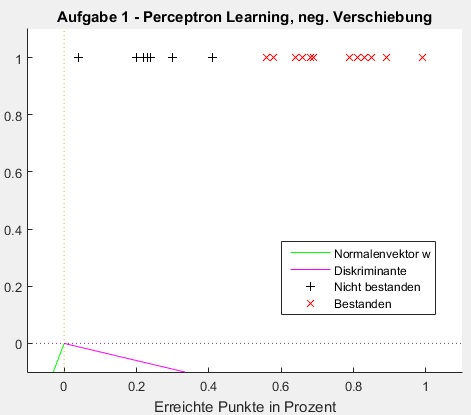
\includegraphics[width=10cm]{a1_01.jpg}\\
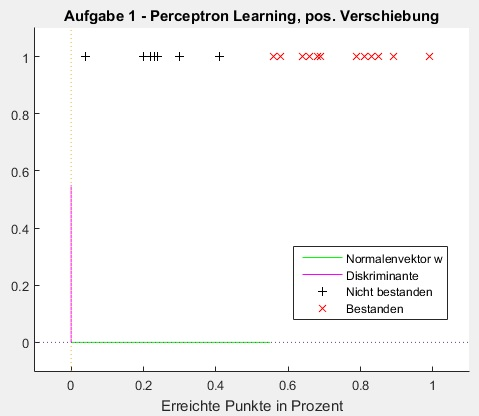
\includegraphics[width=10cm]{a1_02.jpg}
\newpage
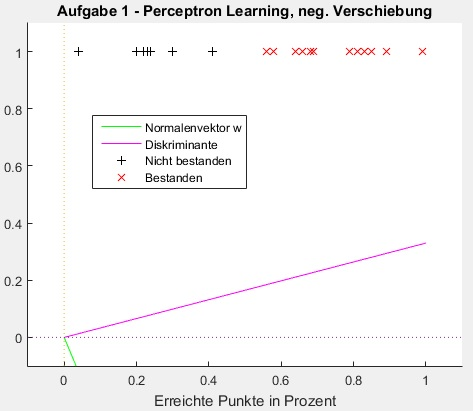
\includegraphics[width=10cm]{a1_03.jpg}\\
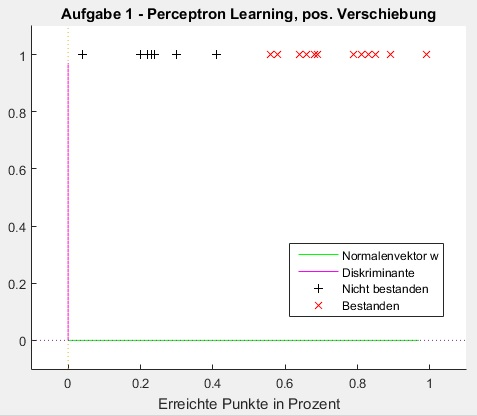
\includegraphics[width=10cm]{a1_04.jpg}
\newpage
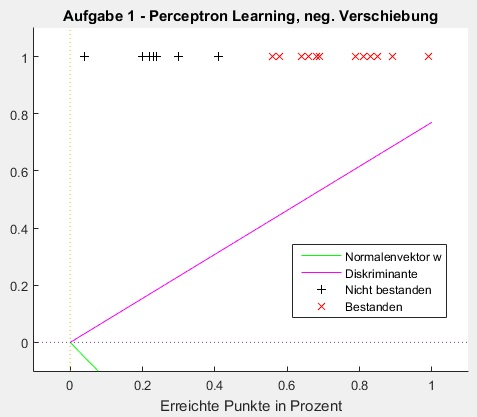
\includegraphics[width=10cm]{a1_05.jpg}\\
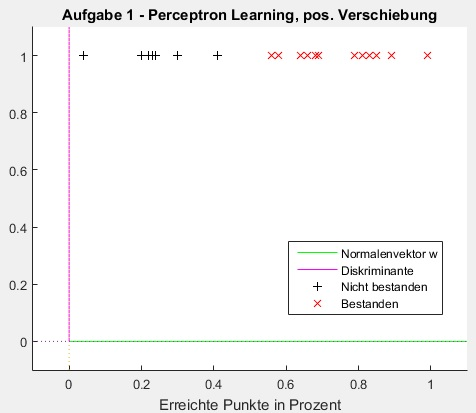
\includegraphics[width=10cm]{a1_06.jpg}
\newpage
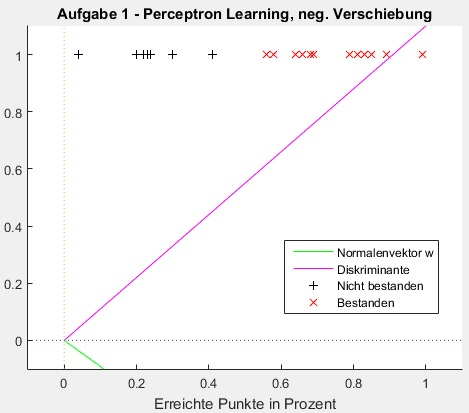
\includegraphics[width=10cm]{a1_07.jpg}\\
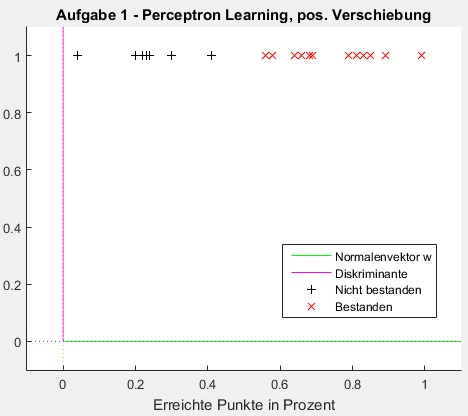
\includegraphics[width=10cm]{a1_08.jpg}
\newpage
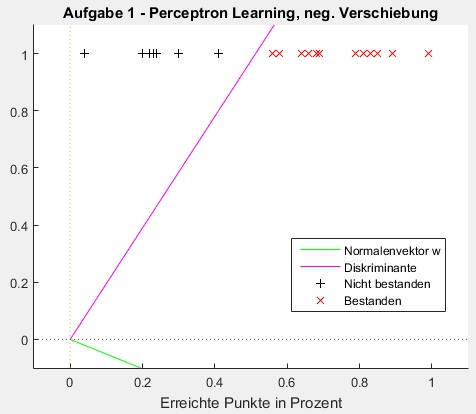
\includegraphics[width=10cm]{a1_09.jpg}
\end{center}

\section{Schwellwerte}

\subsection{Aufgabe 2A}

\begin{lstlisting}[language=Matlab]
schwellwerte = [];
for iter = 1:100
    randOrder = randperm(size(Features, 1));
    randFeatures = Features(randOrder');
    w = [max(Punkte) max(Noten)]; % random choosen vector w
    t = 0;
    limit = size(Data, 1); % number of iterations
    for i = 1:limit
        w_norm = w / norm(w);
        lineNum = mod(i, size(randFeatures,1))+1;
        proj = randFeatures(lineNum, :) * w_norm'; % scalar projection
        if Noten(lineNum) == 1
            if proj < 0
                t = t + 1;
                w = w + randFeatures(lineNum, :);
                diskriminante = [-w(2) w(1)];
            end
        end
        if Noten(lineNum) == 0
            if proj >= 0 % wrong classification
                t = t + 1;
                w = w - randFeatures(lineNum, :);
                diskriminante = [-w(2) w(1)];
            end
        end
    end
    schwellwerte = vertcat(schwellwerte, w);
end

% output
schwellwerte
mean_schwellwert = mean(schwellwerte)
% mean_schwellwert = [-0.1980 -0.1880]
\end{lstlisting}

\newpage

\subsection{Aufgabe 2B}

\begin{lstlisting}[language=Matlab]
figure('NumberTitle','off','Name','Aufgabe 2 - Lin. Regression');

% calculate
onesVector = ones(size(Data,1), 1);
X = horzcat(onesVector, Punkte);
beta = inv(X'*X) * X' * Noten;
fx = beta(1) + beta(2)*x2;
pkt = (0.5-beta(1))/beta(2);
% pkt = 0.4804

% plot
hold on
scatter(Punkte, Noten, 'x', 'b')
plot (x2,fx, 'g')
scatter(pkt,0.5, 'o', 'r')

axis([-0.1 1.1 -0.1 1.1]);
legend('Noten', 'Diskriminante', 'Schwellenwert');
\end{lstlisting}

\begin{center}
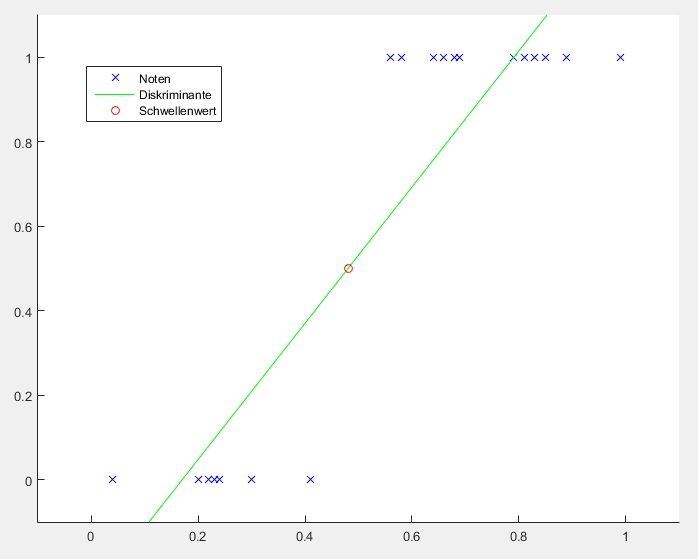
\includegraphics[width=10cm]{a2b.jpg}
\end{center}


\end{document}